\documentclass[a4]{scrartcl}
\usepackage[utf8]{inputenc}
\usepackage{hyperref}
\usepackage{color}
\usepackage{tikz}
\usepackage{pgf}
\usepackage{graphicx}
\usepackage{amsmath, amssymb}
\usepackage{pdfpages}

\newcommand\invisiblesection[1]{%
  \refstepcounter{section}%
  \addcontentsline{toc}{section}{\protect\numberline{\thesection}#1}%
  \sectionmark{#1}}

\begin{document}

\author{Simon Schlepphorst \and Federico Diaz Capriles}
\title{Ising Model}
\subtitle{A Statistical System at Finite Temperature}
\date{16 March 2017}

\maketitle

\begin{abstract}
%TODO
Abstract ...
\end{abstract}

\tableofcontents

\section{Theory}

	\begin{minipage}{.6\textwidth}
			\begin{center}
			
\begin{tikzpicture}
				\draw[step=.5cm,gray,very thin] (0.1,0.1) grid (2.9,2.9);
				\fill[black] (0.1,0.1) rectangle (.5,1.5);
				\fill[black] (0.1,1.5) rectangle (2,2);
				\fill[black] (2,0.1) rectangle (2.5,0.5);
				\fill[black] (1.5,0.5) rectangle (2,1);
				\fill[black] (0.5,1) rectangle (1,1.5);
				\fill[black] (2,2) rectangle (2.9,2.9);
			\end{tikzpicture}
		\end{center}
	\end{minipage}%
	\begin{minipage}[]{.4\textwidth}
		$ \square $ Spin up \\ 
		$ \blacksquare $ Spin down 
	\end{minipage}
	\vspace{-.05cm}
	\begin{equation}
		 \mathcal{H}(\textbf{s}) = -J \sum_{\langle i, j \rangle} s_{i} s_{j}
	\end{equation}
	{\scriptsize \begin{equation*}
		 s_{n} \in \{-1,+1\}
	\end{equation*}}\vspace{-.5cm}
	\begin{equation}
		\textbf{s} = (s_{1}, s_{2}, \dots, s_{N})
	\end{equation}
	\begin{equation}
		\mathcal{Z} = \sum_{\textbf{s}} exp(-\frac{1}{k_{B} T}\mathcal{H}(s))
	\end{equation}
	
\section{Metropolis Algorithm}

\subsection{Results}

\subsection{Problems and Limitations}

\section{Cluster Algorithm}

\subsection{Results}
\pageref{MCT}

\subsection{Problems and Limitations}

\appendix
\invisiblesection{Metropolis Algorithm}
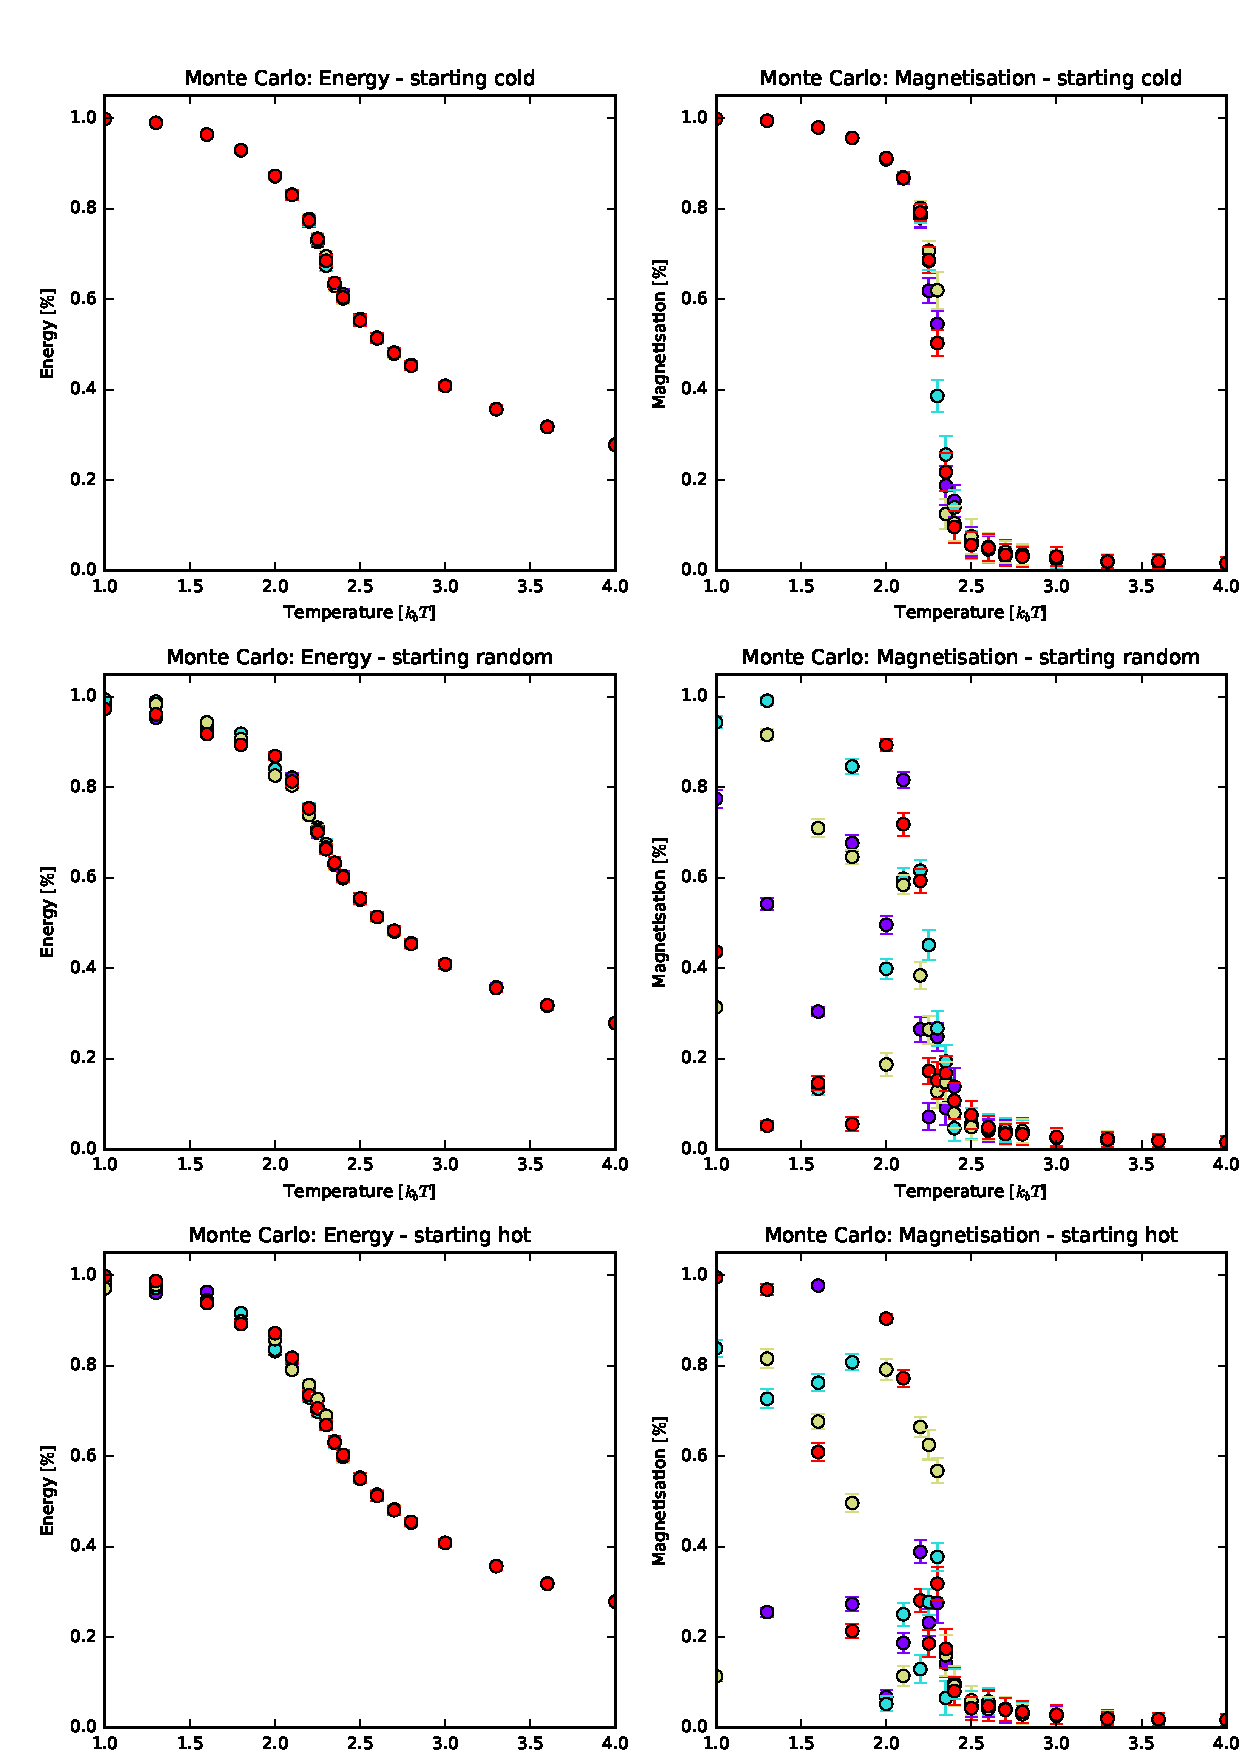
\includepdf[pages={-}, addtotoc={1,subsection,2,Temperature,MCT}, scale=0.9]{_build/Monte-Carlo_Temperatures.pdf}
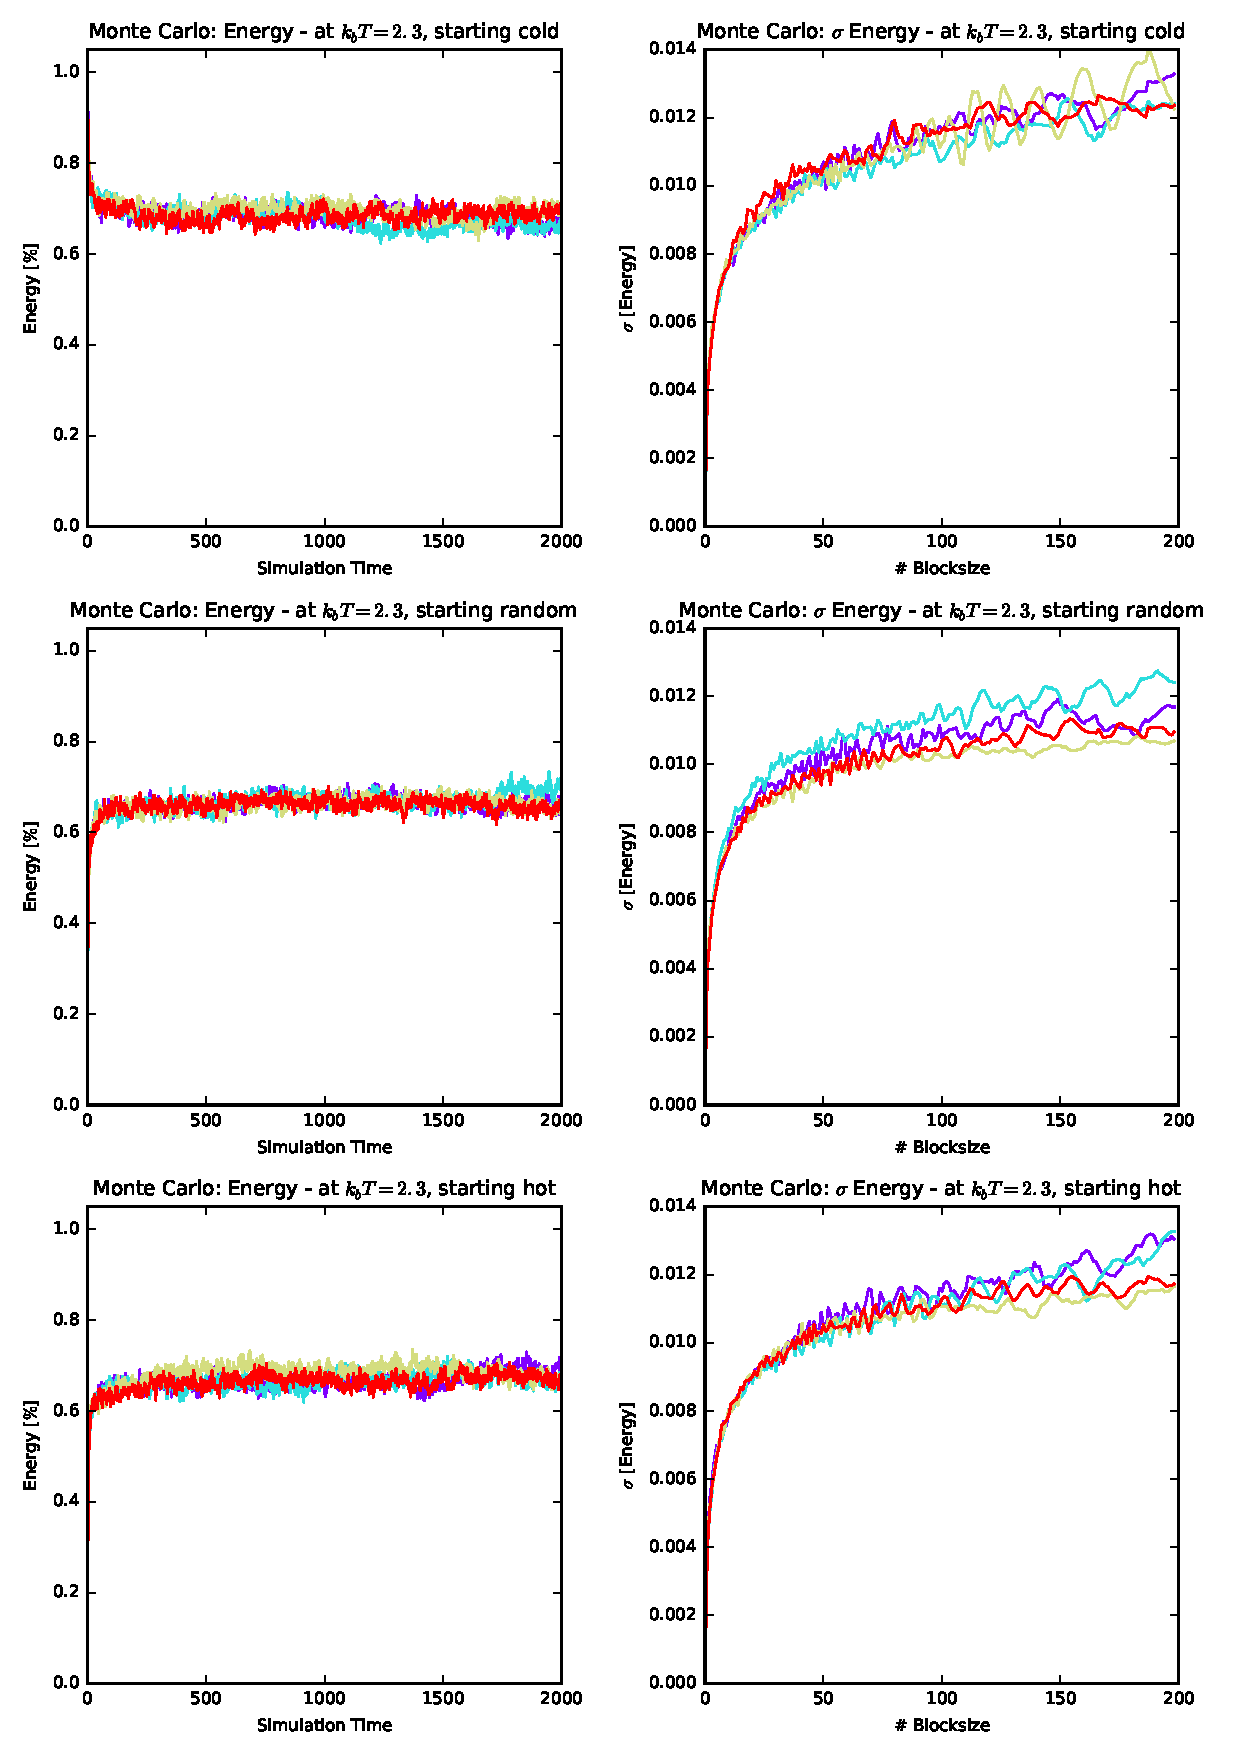
\includepdf[pages={-}, addtotoc={1,subsection,2,Energy,MCE}, scale=0.9]{_build/Monte-Carlo_Energy.pdf}
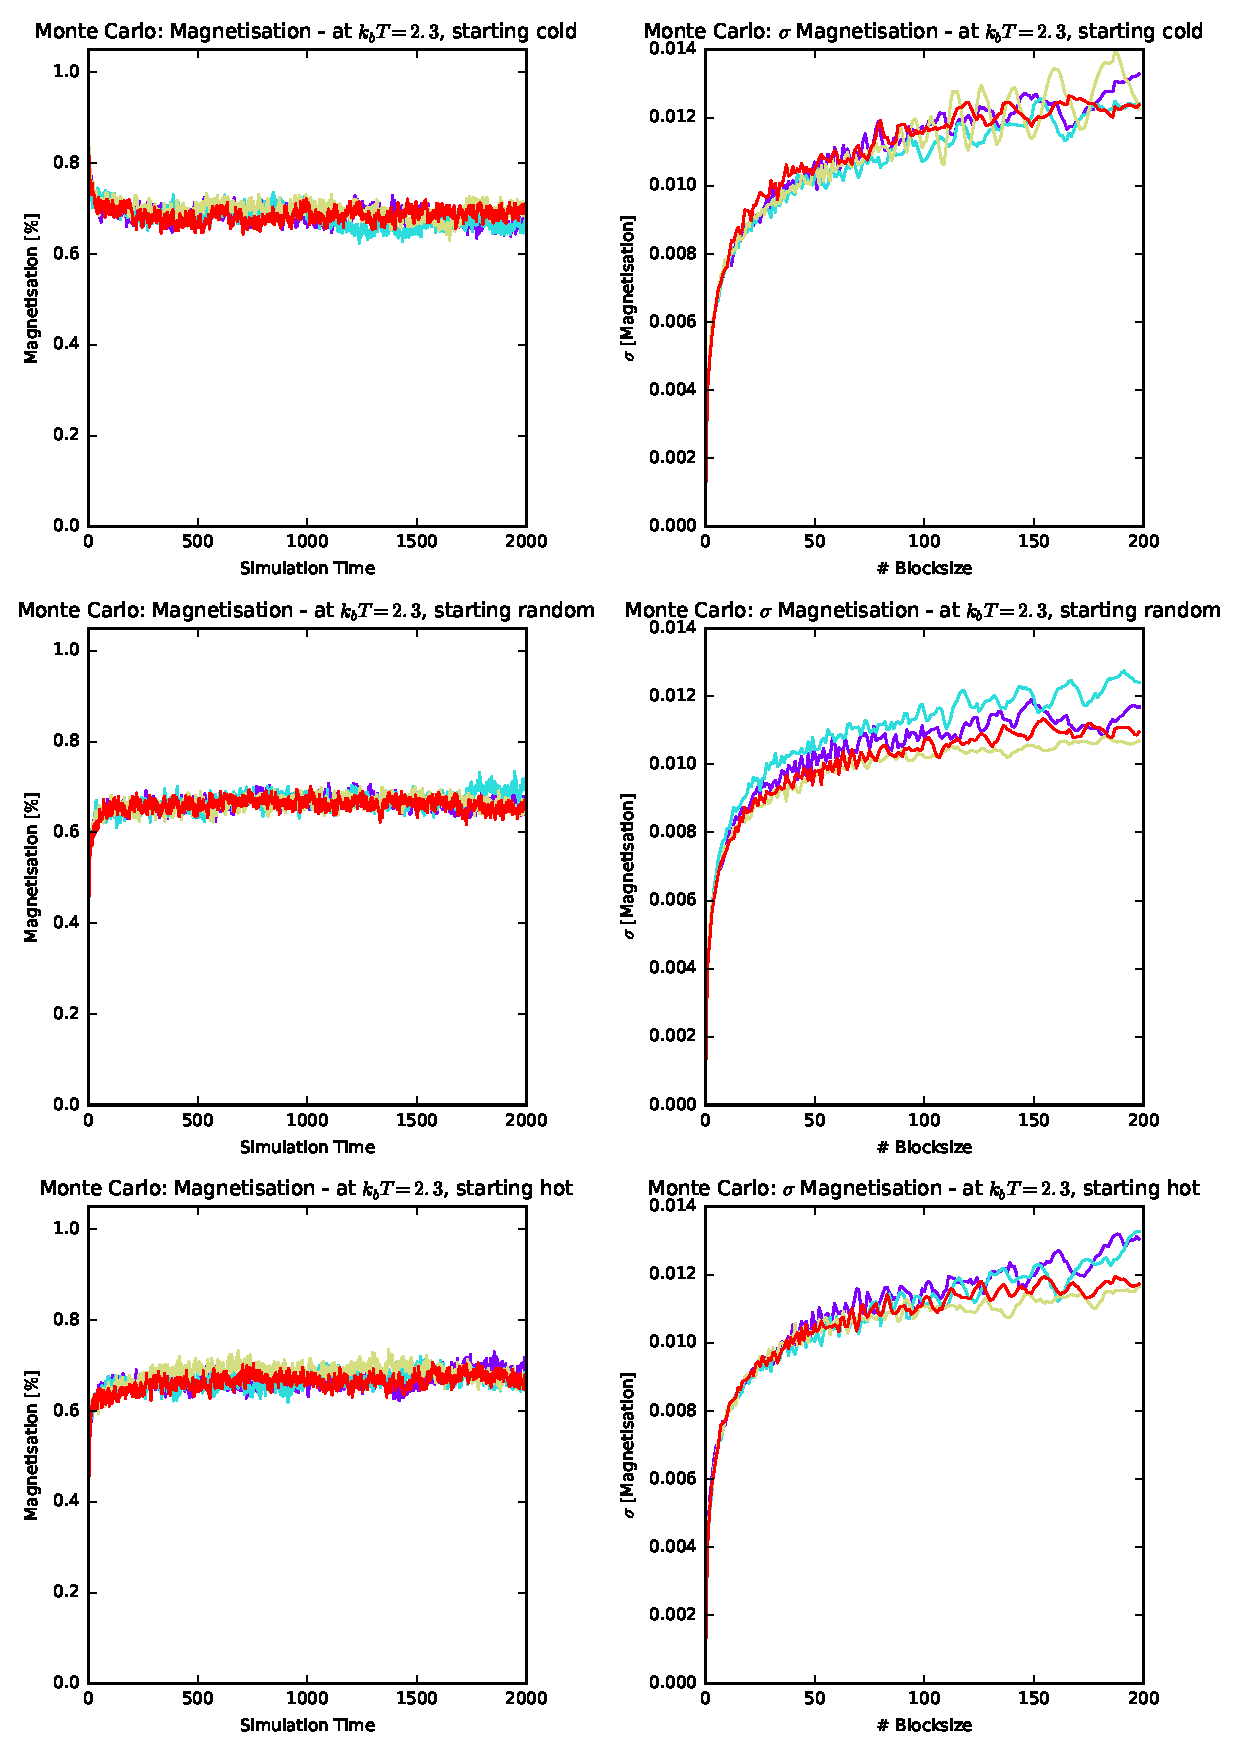
\includepdf[pages={-}, addtotoc={1,subsection,2,Magnetisation,MCM}, scale=0.9]{_build/Monte-Carlo_Magnetisation.pdf}

\invisiblesection{Cluster Agorithm}
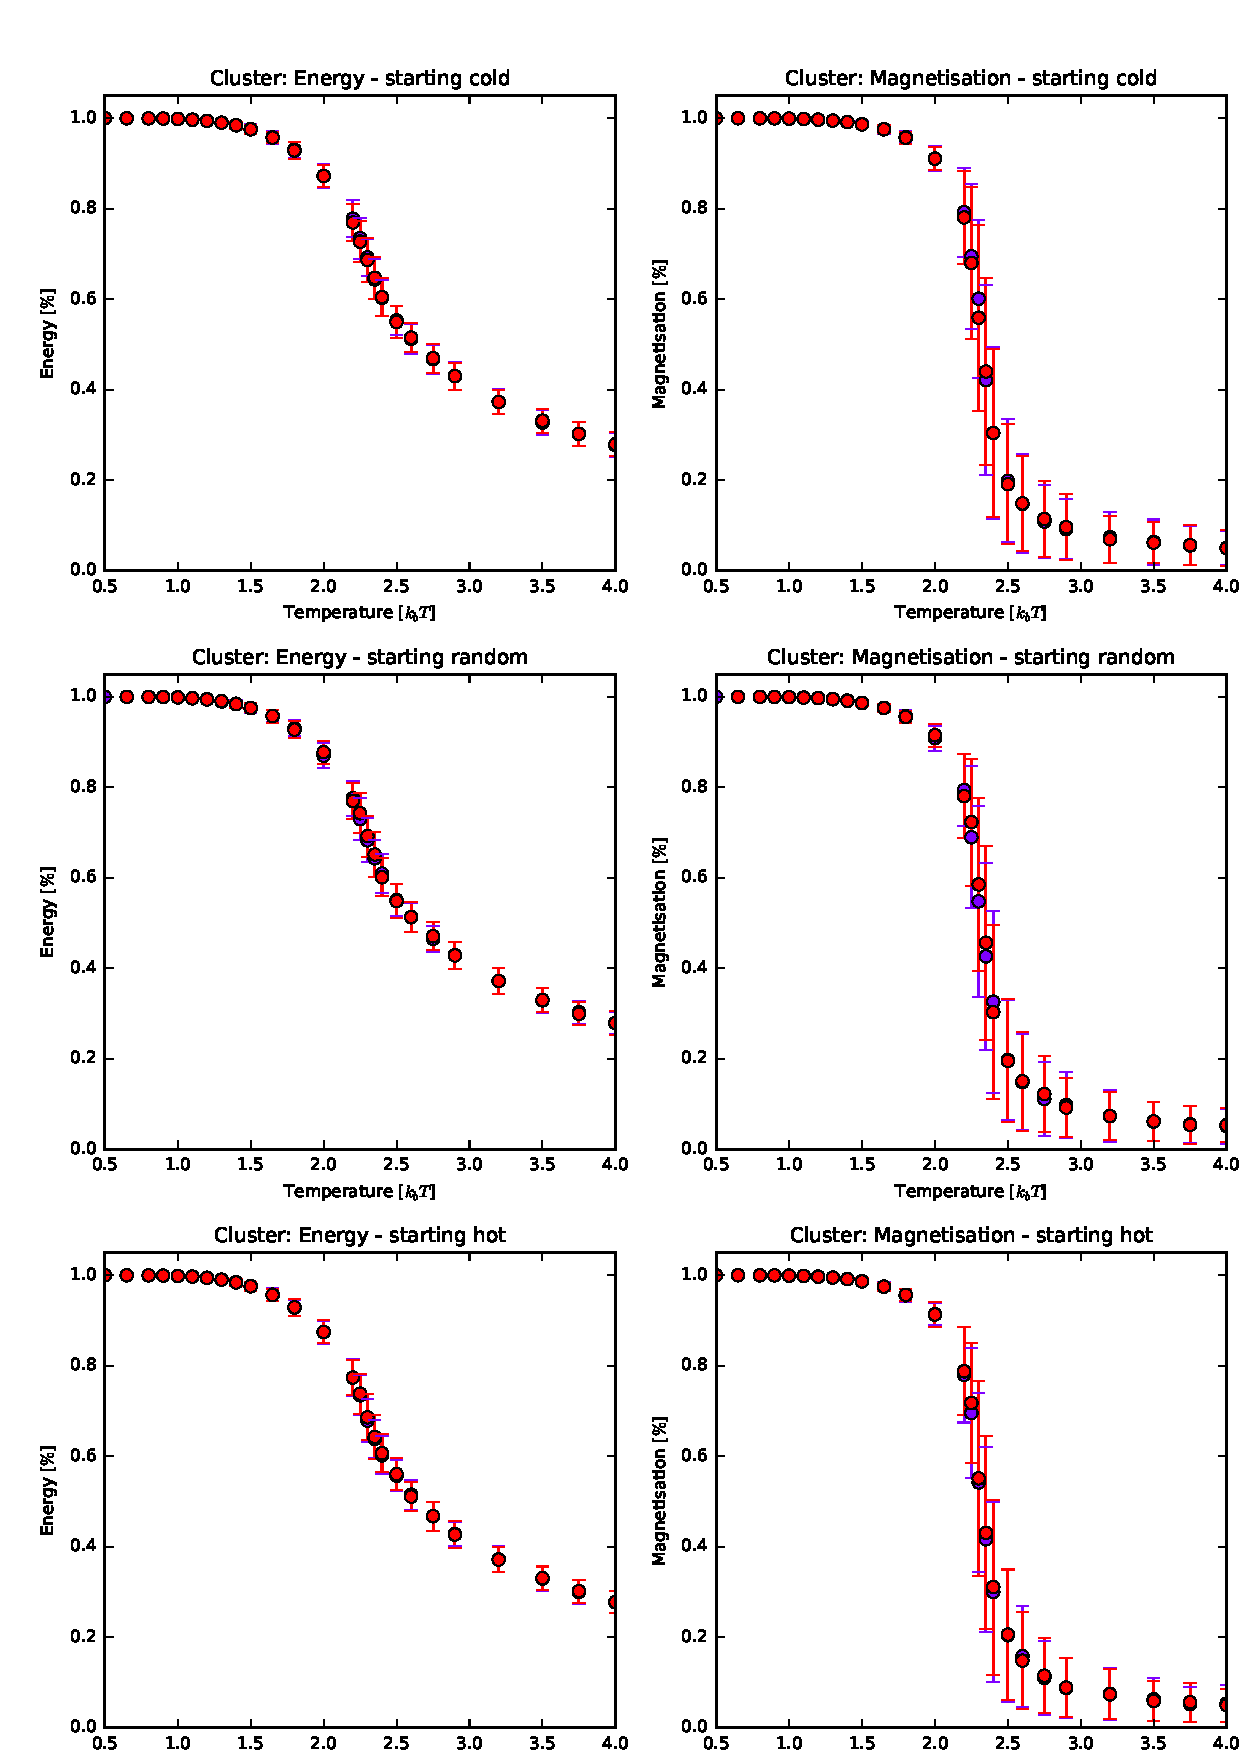
\includepdf[pages={-}, addtotoc={1,subsection,2,Energy,CLT}, scale=0.9]{_build/Cluster_Temperatures.pdf}
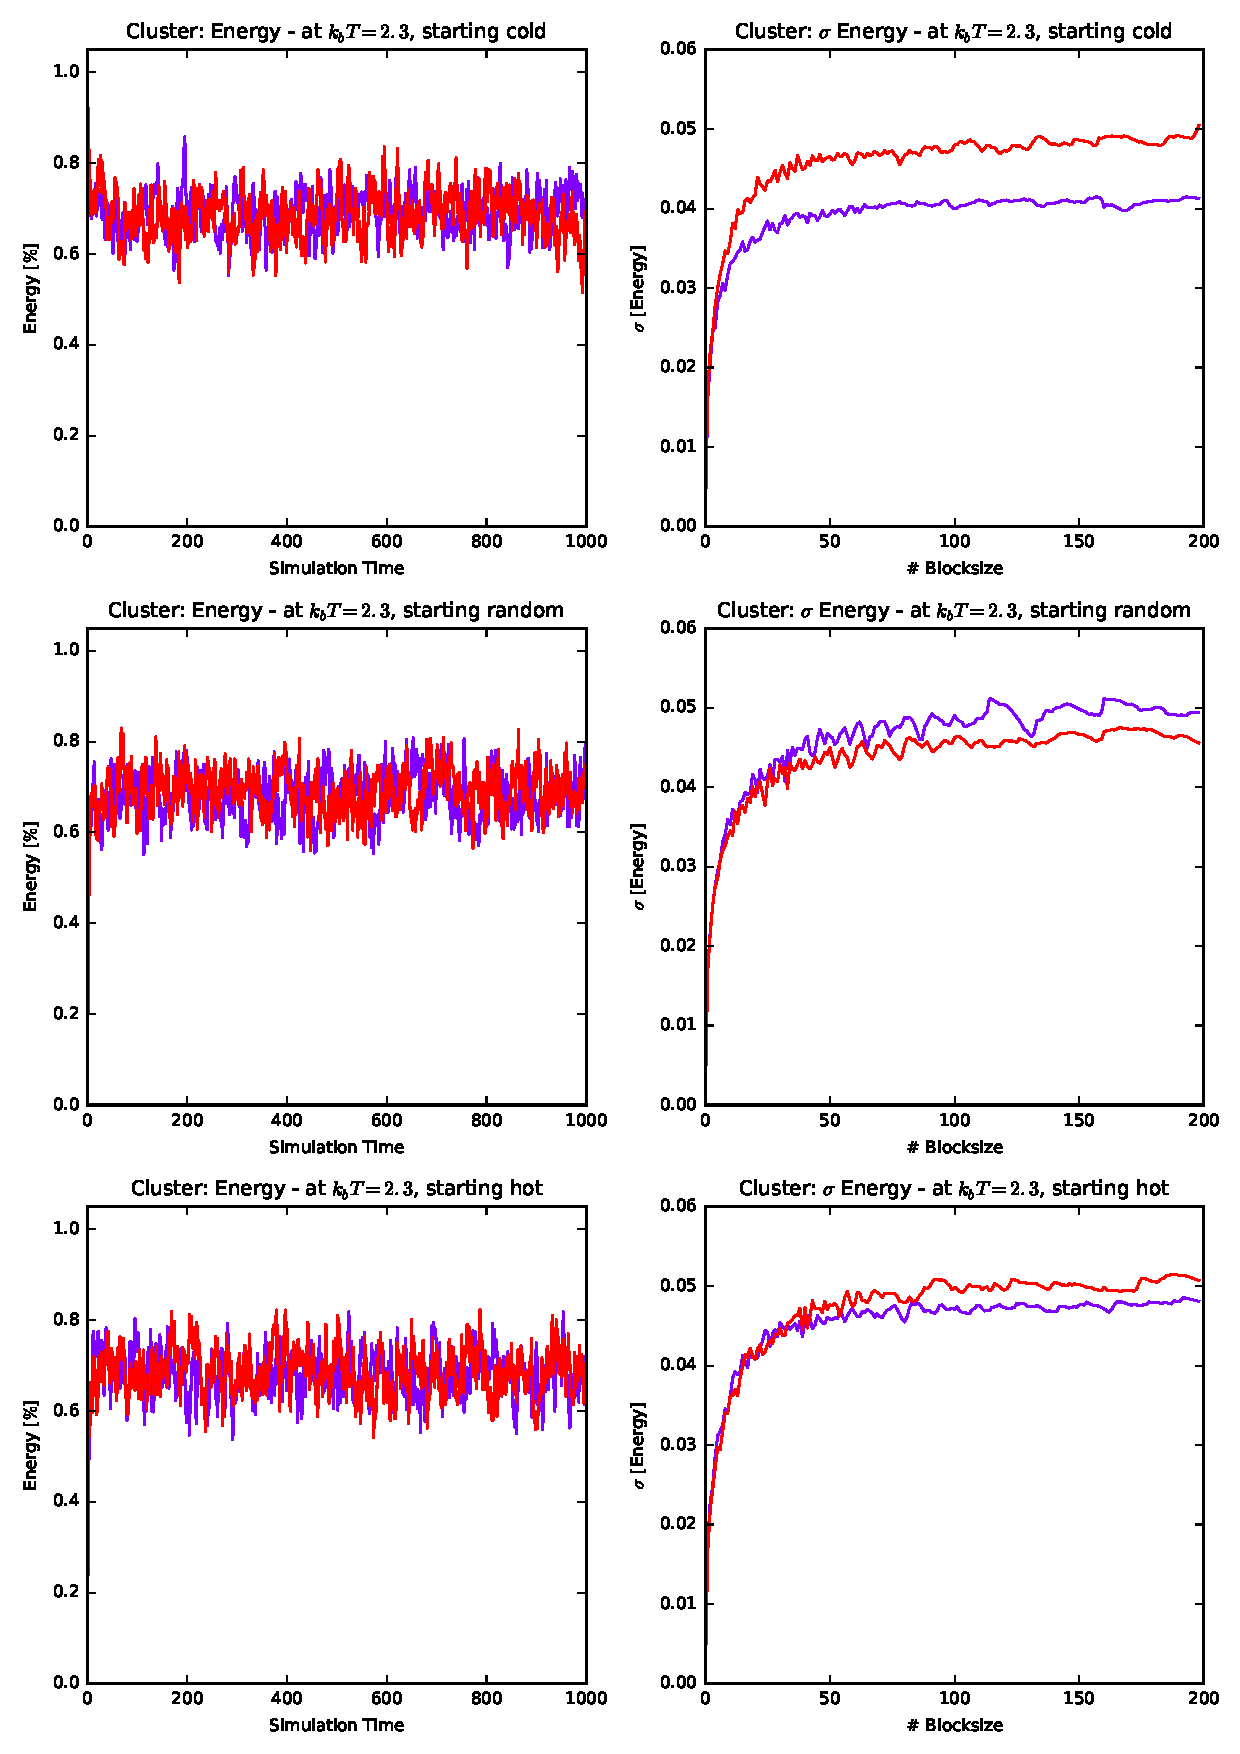
\includepdf[pages={-}, addtotoc={1,subsection,2,Energy,CLE}, scale=0.9]{_build/Cluster_Energy.pdf}
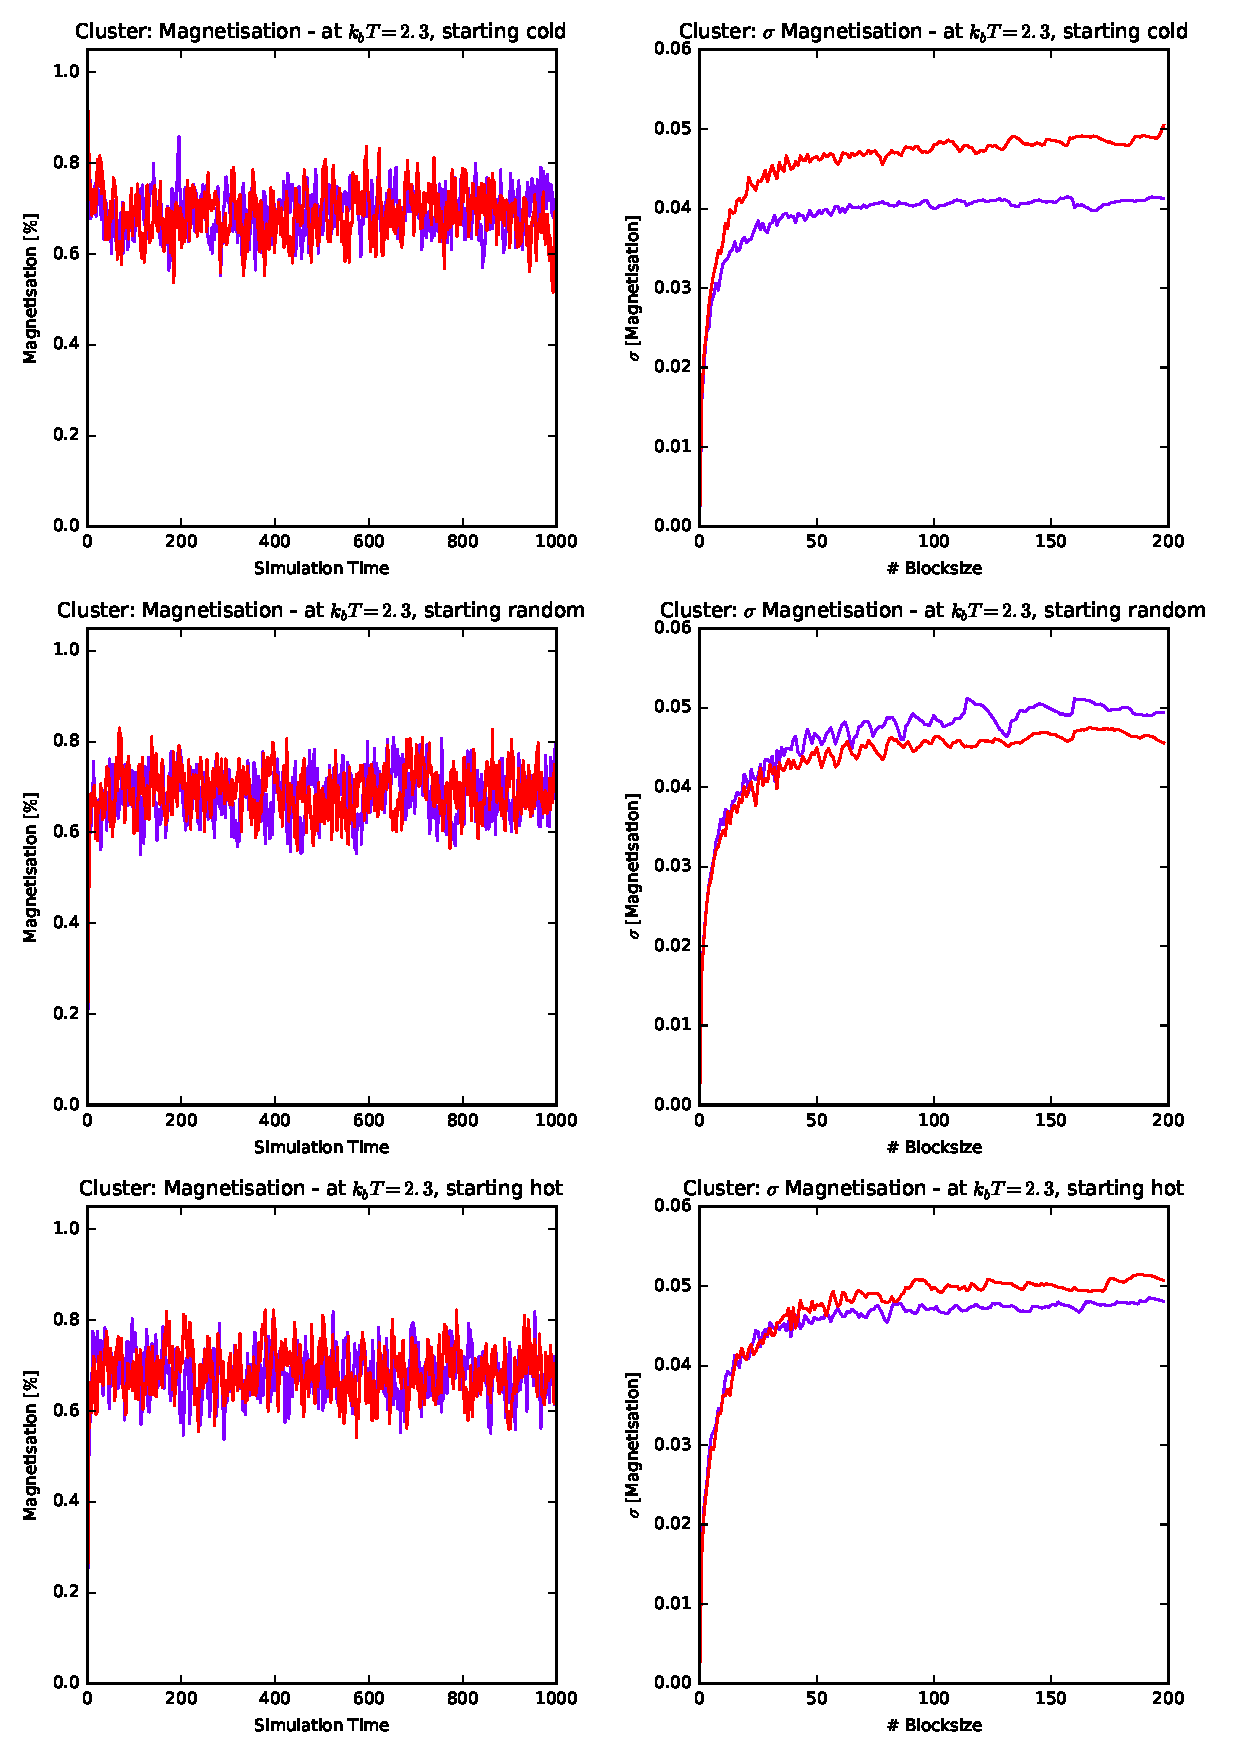
\includepdf[pages={-}, addtotoc={1,subsection,2,Energy,CLM}, scale=0.9]{_build/Cluster_Magnetisation.pdf}

\end{document}
